% Chapter 5

\chapter{Results and discussion} % Main chapter title

\label{Chapter5} % For referencing the chapter elsewhere, use \ref{Chapter5} 
\section{Small Network solved by D-Wave CQM Sampler}
Since the problem we are tackling has just a few variables we can sample all the configuration space. For this task we use the \textit{CQM ExactSolver} class. One of the advantage of CQM is that it writes down if the solution is feasible, i.e.,  if that solution satisfy all the constraints of our problem. The solution of the problem is represented graphically in Figure\,\ref{fig: Green_final}.
\begin{figure}[H]
  \begin{center}
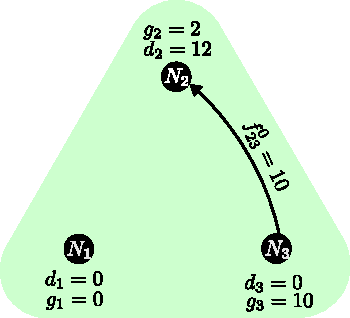
\includegraphics[width=0.4\textwidth]{Figures/Green_Final.pdf}
  \end{center}
  \caption{Graphical solution of three node problem.}
  \label{fig: Green_final}
\end{figure}
Notice that Table\,\ref{tab:SmallNetworkResults} represents only feasible solutions. They are sorted from lower energy to higher energy which means that the first row is the solution that minimizes the objective function by fulfilling the constraints, in this example the demand.
 \begin{table}[H]
\centering
\begin{tabular}{ |c|c|c|c|c|c|c|c| }
  \hline			
  $\mathbf{x_{12}}$ & $\mathbf{x_{13}}$ & $\mathbf{x_{23}}$ & $\mathbf{g_{1}}$ & $\mathbf{g_{2}}$ & $\mathbf{g_{3}}$ & \textbf{Energy} & \textbf{Feasible} \\
  \hline
    0 & 0 & 1 & 0 & 2 & 10 & 60 & True \\
  \hline
    0 & 0 & 1 & 0 & 3 & 9 & 63 & True \\
  \hline
    0 & 0 & 1 & 0 & 4 & 8 & 66 & True \\
  \hline
    0 & 0 & 1 & 0 & 6 & 7 & 69 & True \\
  \hline
\end{tabular}
\caption{D-Wave's feasible solutions to the TEP combinatorial optimization problem.}
\label{tab:SmallNetworkResults}
\end{table}
The optimal solution decides to build the most expensive transmission line, i.e., the one connecting nodes 2 and 3, and to use the maximum capacity of the cheapest generator, the one at node 3, see Table\,\ref{tab:SmallNetwork}.
\subsection{Heuristic Solvers}
If we plan to tackle large problems with a high number of decision variables, we need to use heuristic solvers such as the quantum annealer, the simulated annealing solver or the tabu solver. Otherwise, the required time to sample all the possible combinations of the binary variables is going to be very large. We need to accept sub-optimal solutions to tackle large problems.
%%%%%%%%%%%%%%%%%%%%%%%%%%%%%%%%%%%%%%%%%%%%%%%
\section{Hybrid Approaches of D-Wave}
